\documentclass[11pt]{article}
\usepackage{listings}
\usepackage{tikz}
\usepackage{url}
\usepackage{hyperref}
%\usepackage{algorithm2e}
\usetikzlibrary{arrows,automata,shapes,positioning}
\tikzstyle{block} = [rectangle, draw, fill=blue!20, 
    text width=2.5em, text centered, rounded corners, minimum height=2em]
\tikzstyle{bw} = [rectangle, draw, fill=blue!20, 
    text width=3.5em, text centered, rounded corners, minimum height=2em]

\newcommand{\handout}[5]{
  \noindent
  \begin{center}
  \framebox{
    \vbox{
      \hbox to 5.78in { {\bf ECE459: Programming for Performance } \hfill #2 }
      \vspace{4mm}
      \hbox to 5.78in { {\Large \hfill #5  \hfill} }
      \vspace{2mm}
      \hbox to 5.78in { {\em #3 \hfill #4} }
    }
  }
  \end{center}
  \vspace*{4mm}
}

\lstset{basicstyle=\ttfamily \scriptsize}

\newcommand{\lecture}[4]{\handout{#1}{#2}{#3}{#4}{Lecture #1}}
\topmargin 0pt
\advance \topmargin by -\headheight
\advance \topmargin by -\headsep
\textheight 8.9in
\oddsidemargin 0pt
\evensidemargin \oddsidemargin
\marginparwidth 0.5in
\textwidth 6.5in

\parindent 0in
\parskip 1.5ex
%\renewcommand{\baselinestretch}{1.25}

% http://gurmeet.net/2008/09/20/latex-tips-n-tricks-for-conference-papers/
\newcommand{\squishlist}{
 \begin{list}{$\bullet$}
  { \setlength{\itemsep}{0pt}
     \setlength{\parsep}{3pt}
     \setlength{\topsep}{3pt}
     \setlength{\partopsep}{0pt}
     \setlength{\leftmargin}{1.5em}
     \setlength{\labelwidth}{1em}
     \setlength{\labelsep}{0.5em} } }
\newcommand{\squishlisttwo}{
 \begin{list}{$\bullet$}
  { \setlength{\itemsep}{0pt}
     \setlength{\parsep}{0pt}
    \setlength{\topsep}{0pt}
    \setlength{\partopsep}{0pt}
    \setlength{\leftmargin}{2em}
    \setlength{\labelwidth}{1.5em}
    \setlength{\labelsep}{0.5em} } }
\newcommand{\squishend}{
\end{list}  }
\newtheorem{example}{Example}


\begin{document}

\lecture{12 --- January 30, 2015}{Winter 2015}{Patrick Lam}{version 1}

In class, I live-coded a parallelization
of the Mandelbrot code. I had to first refactor the code, creating
an array to hold the output. Then I added a struct to pass the offset and
stride to the thread. Finally, I invoked pthread to create and join threads.

\section*{Breaking Dependencies with Speculation}
Recall that computer architects often use speculation to predict branch
targets: the direction of the branch depends on the condition codes
when executing the branch code. To get around having to wait, the processor
speculatively executes one of the branch targets, and cleans up if it
has to.

We can also use speculation at a coarser-grained level and
speculatively parallelize code. We discuss two ways of doing so: one
which we'll call speculative execution, the other value speculation.

\subsection*{Speculative Execution for Threads.} The idea here is to
start up a thread to compute a result that you may or may not need.
Consider the following code:

{\small \begin{verbatim}
  void doWork(int x, int y) {
    int value = longCalculation(x, y);
    if (value > threshold) {
      return value + secondLongCalculation(x, y);
    }
    else {
      return value;
    }
  }
\end{verbatim} }
Without more information, you don't know whether you'll have to execute
{\tt secondLongCalculation} or not; it depends on the return value of
{\tt longCalculation}. 

Fortunately, the arguments to {\tt secondLongCalculation} do not
depend on {\tt longCalculation}, so we can call it at any point. 
Here's one way to speculatively thread the work:

{\small \begin{verbatim}
  void doWork(int x, int y) {
    thread_t t1, t2;
    point p(x,y);
    int v1, v2;
    thread_create(&t1, NULL, &longCalculation, &p);
    thread_create(&t2, NULL, &secondLongCalculation, &p);
    thread_join(t1, &v1);
    thread_join(t2, &v2);
    if (v1 > threshold) {
      return v1 + v2;
    } else {
      return v1;
    }
  }
\end{verbatim} }
We now execute both of the calculations in parallel and return the same
result as before.

{\sf Intuitively: when is this code faster? When is it slower? How
  could you improve the use of threads?}\\[4em]

We can model the above code by estimating the probability $p$ that
the second calculation needs to run, the time $T_1$ that it takes
to run {\tt longCalculation}, the time $T_2$ that it takes to run
{\tt secondLongCalculation}, and synchronization overhead $S$.
Then the original code takes time
\[ T = T_1 + p T_2, \]
while the speculative code takes time
\[ T_s = \max(T_1, T_2) + S.\]

\paragraph{Exercise.} Symbolically compute when it's profitable to do the
speculation as shown above. There are two cases: $T_1 > T_2$ and $T_1
< T_2$. (You can ignore $T_1 = T_2$.)

\subsection*{Value Speculation}
The other kind of speculation is value speculation. In this case,
there is a (true) dependency between the result of a computation 
and its successor:
% note: v1 is meant to be the result you get from longCalculation this time, while last_value is what you got last time. (The code doesn't show that). If you get the same result from longCalculation this time as you did last time, then secondLongCalculation is correct and you don't need to redo it.

{\small \begin{verbatim}
  void doWork(int x, int y) {
    int value = longCalculation(x, y);
    return secondLongCalculation(value);
  }
\end{verbatim} }
If the result of {\tt value} is predictable, then we can speculatively
execute {\tt secondLongCalculation} based on the predicted value.
(Most values in programs are indeed predictable).
{\small \begin{verbatim}
void doWork(int x, int y) {
    thread_t t1, t2;
    point p(x,y);
    int v1, v2, last_value;
    thread_create(&t1, NULL, &longCalculation, &p);
    thread_create(&t2, NULL, &secondLongCalculation,
                  &last_value);
    thread_join(t1, &v1);
    thread_join(t2, &v2);
    if (v1 == last_value) {
      return v2;
    } else {
      last_value = v1;
      return secondLongCalculation(v1);
    }
}
\end{verbatim}
}
Note that this is somewhat similar to memoization, except with 
parallelization thrown in. In this case, the original running time is
\[ T = T_1 + T_2, \]
while the speculatively parallelized code takes time
\[ T_s = \max(T_1, T_2) + S + pT_2,\]
where $S$ and $p$ are the same as above.

\paragraph{Exercise.} Do the same computation as for speculative execution.

\subsection*{When can we speculate?}
Speculation isn't always safe. We need the following conditions:
  \begin{itemize}
    \item {\tt longCalculation} and {\tt secondLongCalculation} must not call
      each other.
    \item {\tt secondLongCalculation} must not depend on
      any values set or modified by {\tt longCalculation}.
    \item The return value of {\tt longCalculation} must be deterministic.
  \end{itemize}

As a general warning: Consider the \emph{side effects} of function calls.

\section*{Critical Paths}
You should be familiar with the concept of a critical path from previous
courses; it is the minimum amount of time to complete the task, taking
dependencies into account, and without speculating.

Consider the following diagram, which illustrates dependencies between
tasks (shown on the arrows). 
Note that B depends on A, and D depends on B and C, but C does
not depend on anything, so it could be done in parallel with
everything else. You can also compute expected execution times
for different strategies.
\begin{center}
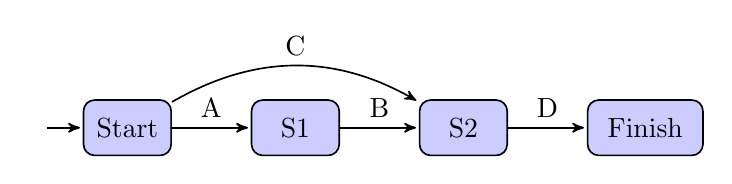
\begin{tikzpicture}[->,>=stealth',shorten >=1pt,auto,column sep=2.2cm,
                    semithick,initial text=]
  \node[initial,block] (s0) {Start};
  \node[block] (s1) [right=of s0] {S1};
  \node[block] (s2) [right=of s1] {S2};
  \node[bw] (s3) [right=of s2] {Finish};

  \path (s0) edge node {A} (s1)
        (s1) edge node {B} (s2)
        (s2) edge node {D} (s3)
        (s0) edge[bend left=30] node {C} (s2);
\end{tikzpicture}
\end{center}

\section*{Data and Task Parallelism}
There are two broad categories of paralellism: data parallelism and
task parallelism. An analogy to data parallelism is hiring a call
center to (incompetently) handle large volumes of support calls,
\emph{all in the same way}. Assembly lines are an analogy to task
parallelism: each worker does a \emph{different} thing.

More precisely, in data parallelism, multiple threads perform the
\emph{same} operation on separate data items. For instance, you have a
big array and want to double all of the elements. Assign part of the
array to each thread. Each thread does the same thing: double array
elements.

In task parallelism, multiple threads perform \emph{different}
operations on separate data items. So you might have a thread that
renders frames and a thread that compresses frames and combines them
into a single movie file.

We'll continue by looking at a number of parallelization patterns,
examples of how to apply them, and situations where they might apply.

\subsection*{Data Parallelism with SIMD}
We'll talk about single-instruction multiple-data (SIMD) later on in
this course, but here's a quick look. Each SIMD
instruction operates on an entire vector of data. These instructions
originated with supercomputers in the 70s. More recently, GPUs; the
x86 SSE instructions; the SPARC VIS instructions; and the
Power/PowerPC AltiVec instructions all implement SIMD.

\paragraph{Code.} Let's look at an application of SIMD instructions.

\begin{verbatim}
void vadd(double * restrict a, double * restrict b, int count) {
  for (int i = 0; i < count; i++)
    a[i] += b[i];
}
\end{verbatim}

Compiling this without SIMD on a 32-bit x86 ({\tt gcc -m32 -march=i386 -S}) might give this:
\begin{verbatim}
loop:
  fldl  (%edx)
  faddl (%ecx)
  fstpl (%edx)
  addl  8, %edx
  addl  8, %ecx
  addl  1, %esi
  cmp   %eax, %esi
  jle   loop
\end{verbatim}

We can instead compile to SIMD instructions ({\tt gcc -m32 -march=prescott -mfpmath=sse})
and get something like this:
\begin{verbatim}
loop:
  movupd (%edx),%xmm0
  movupd (%ecx),%xmm1
  addpd  %xmm1,%xmm0
  movpd  %xmm0,(%edx)
  addl   16,%edx
  addl   16,%ecx
  addl   2,%esi
  cmp    %eax,%esi
  jle    loop
\end{verbatim}
The \emph{packed} operations ({\tt p}) operate on multiple data
elements at a time (what kind of parallelism is this?)
The implication is that the loop only needs to loop half as many times.
Also, the instructions themselves are more efficient, because they're
not stack-based x87 instructions.

SIMD is different from the other types of parallelization we're
looking at, since there aren't multiple threads working at once.
It is complementary to using threads, and good for cases
where loops operate over vectors of data. These loops could also be
parallelized; multicore chips can do both, achieving high throughput.
SIMD instructions also work well on small data sets, where thread startup
cost is too high, while registers are just there to use.
\end{document}
